\documentclass[11pt,
bibtotoc,liststotoc,appendixprefix
oneside,paper=a4,headings=small, twoside=false]{scrbook}
%
% Packages
% -----------------------------------
\usepackage[
  paper=a4paper,
  left=20mm,
  right=25mm,
  top=25mm,
  bottom=50mm,
  bindingoffset=10mm]{geometry}		% Seitenr�nder und Bindungskorrektur einstellen




%\usepackage{apacite} 				% Literatur-Referenzen: American Psycholog. Assoc.
%\usepackage{natbib}	
\usepackage[square, numbers]{natbib}			
\usepackage{amsthm}	
%\usepackage[dvipsnames]{xcolor} %color for tables
\usepackage[nopostdot,style=super,nonumberlist,toc,automake]{glossaries}
\makeglossaries					%Load glossery package for abbreviations

%Vielleicht besser alphabetisch ordnen!
\newglossaryentry{resp.}{name={resp.},description={respectively}}
\newglossaryentry{e.g.}{name={e.g.},description={exempli gratia}}
\newglossaryentry{CSV}{name={CSV},description={Comma Seperated Values}}
\newglossaryentry{DREAM}{name={DREAM},description={Dialogue on Reverse Engineering Assessment and Methods}}
\newglossaryentry{mRNA}{name={mRNA},description={messanger RiboNucleotide Acid}}
\newglossaryentry{RTK}{name={RTK},description={Receptor Tyrosin Kinases}}
\newglossaryentry{PPI}{name={PPI},description={protein protein interaction}}
\newglossaryentry{ATP}{name={ATP},description={adenosin triphosphat}}
\newglossaryentry{GRN}{name={GRN},description={Gene regulatory network}}
\newglossaryentry{RPMA}{name={RPMA},description={Reverse phase Protein lysate MicroArray}}
\newglossaryentry{SDS-PAGE}{name={SDS-PAGE},description={Sodium Dodecyl Sulfate - Polyacrylamide Gel Electrophoresis}}
\newglossaryentry{ELISA}{name={ELISA},description={Enzymatic Immunoassay}}
\newglossaryentry{SIF}{name={SIF},description={Standard Interchange Format}}
\newglossaryentry{IG}{name={IG},description={Interaction Graph}}
\newglossaryentry{STG}{name={STG},description={State Transition Graph}}
\newglossaryentry{MAP}{name={MAP},description={Mitogen Activated Protein}}

%\setcitestyle{round,aysep={}} 		% Indizierg. in runden Klammern, zw. Autor u. Jahr
\setcitestyle{square}
%\usepackage[latin1]{inputenc} 		% Umlaute im Text
%\usepackage{ngerman}				% Rechtschreibg.
\usepackage[T1]{fontenc}
\usepackage{lmodern}				% Schriftfamilie
\usepackage{microtype}				% f�r die Mikrotypografie (besseres Schriftbild)
\usepackage[headsepline,footsepline]{scrpage2}
%\usepackage{subcaption} 
\usepackage[english]{babel}

\usepackage{graphicx} 				% Grafiken einf�gen (pdf,png - aber jpg vermeiden)
\graphicspath{{./Bilder/}}          % Pfad zu den Bildern
\usepackage[export]{adjustbox}		% Positionieren von Bildern Tabellen
\usepackage{subfigure}				% L�sst Bilder nebeneinander darstellen
\usepackage{varwidth}
\usepackage{url}					% URL's formatieren (z.B. in Literatur) 
\usepackage[colorlinks,linkcolor=black,citecolor=black,urlcolor=black]{hyperref} 				% f�r Hyperlinks in PDF-Dokumenten
\usepackage{wrapfig}   
  
\usepackage{tabularx} 				% bessere Gestaltung von Tabellen
\usepackage{longtable} 		
\usepackage{multicol}				
\usepackage{multirow}
\usepackage{booktabs}
\usepackage{tabu}
\usepackage{float}
\usepackage{framed}
\usepackage[labelfont=bf]{caption}
\captionsetup{format=plain, font=small, labelfont=bf}
\usepackage{rotating}
%\usepackage{floatrow}
\usepackage{sidecap}
\sidecaptionvpos{figure}{t}

\usepackage[table]{xcolor}

		
\usepackage[active]{srcltx}

\usepackage{listings}				% Algorithmen

\usepackage{mdwlist}				% Listen

\usepackage{setspace} 				% Zeileneinstellung
\newtheorem{mydef}{Merksatz}  		% Falls Beispiele, Merks�tze m. fortl. Nr. gebr. werden
\newtheorem{bsp}{Beispiel}

\usepackage{todonotes}				% zum Erstellen von ToDos im Editor

\usepackage{lscape}					% zum Rotieren von Seiten

\usepackage{amsmath}				% zum Schreiben von mathematischen Formeln

\usepackage{calc}

\usepackage{scrpage2}
\cfoot[]{}
\ofoot[\pagemark]{\pagemark}
\pagestyle{scrheadings}

%\usepackage{fancyhdr}

\usepackage{footnote}				% Fu�noten
\usepackage{tablefootnote}			% Fu�noten in Tabellen
\usepackage{amssymb}
%\clubpenalty = 10000
%\widowpenalty = 10000 \displaywidowpenalty = 10000

\hyphenation{voll-st\"andigen}		% Worttrennungen global definieren

\setcounter{tocdepth}{3}			% Ebenen, die im Inhaltsverzeichnis angezeigt werden

\theoremstyle{plain}
\newtheorem{thm}{Theorem}[chapter] % reset theorem numbering for each chapter

\theoremstyle{definition}
\newtheorem{defn}[thm]{Definition} % definition numbers are dependent on theorem numbers
\newtheorem{exmp}[thm]{Example} % same for example numbers

% Document
% -----------------------------------
\begin{document}
\parindent 0pt

\frontmatter 
    % Titelseite soll keine Kopf oder Fu�zeile haben
\thispagestyle{empty}

% Alle Elemente sollen zentriert sein


\begin{center}

\vspace*{-10mm}

%{\LARGE Freie Universit�t zu Berlin}\\

\vspace*{1cm}

\includegraphics[width=1.0\textwidth]{FULogo_Ausdruck_RGB}

\vspace*{1cm}

% Art der Arbeit => (Bachelorarbeit ,Diplomarbeit, Masterarbeit, Seminararbeit)
\Large \textbf{Masterthesis}\\ 

%\section*{\Large Masterthesis}

\vspace{1cm}

% Titel der Arbeit 
\LARGE \textbf{Inference of Boolean Networks considering real-life time 
course Data}\\ 

%\mdseries{Inference of Boolean Networks considering real-life time course Data}
%IBM Plex Serif Thin [OTF or TTF only] 

\vspace{1.5cm}

\Large Nina Valery Kersten\\


\parbox{120mm}{
\begin{large}
\begin{tabbing}
\textbf{Supervisors}\\\\
\hspace{.7cm} \= Prof. Dr. Heike Siebert\\
\hspace{.7cm} \= Prof. Dr. Alexander Bockmayr\\\\

\textbf{Advisor}\\\\
Phd. Robert Schwieger\\\\

\textbf{November 20, 2018} \\ 
\end{tabbing}
\end{large}
}

\end{center}
\clearpage{\pagestyle{empty}\cleardoublepage}
 			% Titelblatt
    \newpage
\thispagestyle{empty}

\begin{Large}\textbf{Declaration of Originality}\end{Large}\\

\begin{large}

\vspace*{2cm}

\noindent
I hereby declare that this thesis and this work reported herin was composed by and originated entirely from me. Information derived from published and unpublished work of others has been acknowledged in the text and references are given in the list of sources.

\vspace{2cm}

\noindent
Berlin, November 20,2018\\

%\vspace{3cm}

%\hspace*{7cm}%
%\dotfill\\
%\hspace*{8.5cm}%
Nina Valery Kersten

\end{large}

    \newpage
    \clearpage{\pagestyle{empty}\cleardoublepage}
 

    \onehalfspacing        
              	% Zeilenabstand ab hier 1.5 zeilig
    \tableofcontents 					% Inhaltsverzeichnis
    \clearpage{\pagestyle{empty}\cleardoublepage} 
  
    
    \listoffigures 					 	% Abbildungsverzeichnis
    \clearpage{\pagestyle{empty}\cleardoublepage}
    
    \listoftables						% Tabellenverzeichnis rein
    \clearpage{\pagestyle{empty}\cleardoublepage}
    
    \onehalfspacing
	\printglossary[title={List of Abbreviations}]

	\thispagestyle{empty}


\vspace*{1cm}

\begin{center}
    \textbf{Abstract}
\end{center}

\vspace*{1cm}

\noindent 
%Give a short overview:
%Describe the Pipeline


	\newpage
    \clearpage{\pagestyle{empty}\cleardoublepage}

% -----------------------------------
\mainmatter 							% die einzelnen Kapitel
 	\chapter{Introduction}

The development and functioning of a cell and an organism in general is a product of a complex cellular machinery. This machinery is compound by the interaction of genes, proteins, mRNA and many other substances to induce a cascade of extracellular signals transducted by mechanisms of the cell membrane,reaching the nucleus of the cell, initiating a transcription process that controls the production and abundance of proteins. Proper functioning of these networks is essential to the survival and adapation of all living organisms, while malfunctioning of these networks has been identified as the cause of various diseases \citep{An evaluation of methods for inferring boolean network from time-series data}.
To understand the behaviour of a biological system it is necessary to find and analyze the main important processes in a system in a dynamical manner. Therefore high-throughput techniques provide a big abundance of information about various biological interactions measured over a series of time. Biological information can be considered as different systems such as signal transduction, gene regulation, protein-protein-interaction or metabolism. These information are put in a network which can be yielded by several strategies like Baysian networks, Boolean regulatory networks, Ordinary differential equation models and Neural networks\citep{SAADATPOUR20133}.Once a network is constructed further anaylsis of the network by validating the network (e.g. pertubations like gene manipulation and external treatments, reductions etc.)can be done to figure out the main interactions whose disfunctions cause diseases.
This work is focused on the inference of a Boolean regulatory network, which is helpful to applicate tools like PyBoolNet and BoolFilter for further analysis of the inferenced network. This chapter describes the different kinds of biological data, what a Boolean Regulatory Network is as well as the algorithms to yield a network and how the performance of a algorithm can be measured.


\section{Biological Background}

Depending on the aim of a network inference the biological input data can be depicted by the interaction of proteins, genes and metabolic substances. In this section the intention of using different types of input data is explained and what potentially will be the occuring problems. Different types of biological input data provide different structures of the input data for further network inference algorithms. 
\newpage

\subsection*{Signal Transduction}

In the developement of multicellular organisms the action of extracellualr growth factors activate a cascade of intracellular signaling pathways. These pathways regulate major aspects of cell regulation like cell profileration, cell migration, cell differentiation,cell survival and cell death. To understand the developement of diseases (e.g. cancer) major prozesses (e.g. phosphorylation, ubiquitylation, methylation, etc.) of signal transduction pathways can be delightet by the prediction of a network . In signal transduction proteins are the nodes and directed edges represent interaction, where the biochemical modification of the regulatee is changed by the impact of the regulator. The concentration of signalling pathway underlies high fluctuation over time due to transcriptional and translational regulation, such that the inference of a network is a challenging task \citep{BIES:BIES20834}
%\citep{https://www.ncbi.nlm.nih.gov/pmc/articles/PMC3436851/}.


\begin{figure}[H]
\centering
%\setlength{\abovecaptionskip}{0pt}
\includegraphics[width=0.5\textwidth]{./Bilder/signaltransduction.pdf}
\setlength{\abovecaptionskip}{-10ex}
\caption[Signal Transduction]{\textbf{Signal Transduction.} An environmental signal (e.g. hormone) interacts with a cellular component, most often a cell-surface receptor. The information that the signal has arrived is then converted into other chemical forms, or transduced. The signal is often amplified before introducing a response. Feedback pathways regulate the entire signaling process.\citep{Berg JM, Tymoczko JL, Stryer L. Biochemistry. 5th edition. New York: W H Freeman; 2002. Chapter 15, Signal-Transduction Pathways: An Introduction to Information Metabolism. Available from: https://www.ncbi.nlm.nih.gov/books/NBK21205/} }
%\setlength{\belowcaptionskip}{0pt} 
\label{fig:Fig.1.}
\end{figure}

\newpage
\subsection*{Transcriptional Gene Regulatory Networks}

In a Transcriptional Gene regulatory network (GRN) the nodes are depicted by the genes and the arcs are directed and show whether a gene produces RNA (transcript of the source gene,resp. regulator) which inhibits oder activtes the target gene (regulatee). For network inference computational algorithms take the mRNA expression levels of genes as the input data. In order to determine the appropriate nodes of the network some statistical classification of the mRNA expression level data has to be done. The modelling of a transcriptional gene regulatory network ist done by algorithms like Baysian networks, Boolean regulatory networks, Ordinary differential equation models and Neural networks regression %\citep{https://www.nature.com/articles/nrm2503}.


\begin{figure}[H]
\centering
%\setlength{\abovecaptionskip}{0pt}
\includegraphics[width=0.7\textwidth]{./Bilder/Gene_Regulatory_Network_-_original}
\caption[Transcriptional Gene Regulatory Network (GRN)]{\textbf{Transcriptional Gene Regulatory Network (GRN).}In this example two different signals have an impact of a single target gene. Signal molecule A triggers the conversion of inactive transcription factor A (green oval) into an active form that binds directly to the target gene's cis-regulatory sequence. The process for signal B is more complex. Signal B triggers the separation of inactive B (red oval) from an inhibitory factor (yellow rectangle). B is then free to form an active complex that binds to the active A transcription factor on the cis-regulatory sequence. The net output is expression of the target gene, leveled by A nd B. Thus cis-regulatory DNA sequences with the proteins that assemble on them, integrate information from multiple signaling inputs to produce mRNA-Output . 
\citep{https://public.ornl.gov/site/gallery/detail.cfm?id=302&topic=&citation=&general=gene20regulatory20network&restsection=all} }
%\setlength{\belowcaptionskip}{0pt} 
\label{fig:Fig.2.}
\end{figure}

\newpage

\subsection*{Protein-Protein-Interaction}
In contrast to the gene regulatory interaction network the protein-protein interactions (PPIs) act directly among themselve. Thus the nodes in a network are the interacting proteins. Proteins interact by physical contacts(e.g. electrostatic forces) of high specificity. PPIs play a big role in electron transfer,signal transduction, transport across membranes and cell metabolism. A variety of techniques are known to detect PPIs. The most applicated ones are immuno-precipitations and the yeast two-hybrid approach. The two-hybrid assay is not a relieable indication that two proteins interact \textit{in vivo},because the two interacting proteins are overexpressed.Thus the interaction may not be present in the wild type cells where the concentrations may be significantly lower. For this reason additional information are included to figure out the occurence of true interaction, such as cellular localization and mRNA expression level. The underlying assumption is that true interactions are likelyto occur between proteinsinvolved in the same biological process, proteins found in the same cell compartment, and proteins whose mRNA are coexpressed.
For the identification of protein complexes affinity purification technique is used followed by mass spectrometry (MS) to sequence the proteins in the complexes. The detection of interactions of protein with DNA is done by chromatin immunoprecipitation (ChIP) in addition with expression microarrays, so-called ChIP on Chip approach. This method provide information about the interaction of transcription factors with DNA and the binding sites of transcription factors. Furthermore computational methods are included to predict the protein interactions by protein fusion and using phylogenetic analysis. Interaction networks of PPIs may depict how drug- protein interactions lead to toxic side effects.
%\citep{10.1371/journal.pcbi.1000807}
\citep{doi:10.1586/14789450.1.2.239}

\subsection*{Metabolic Interaction}
Metabolic interactions represent the most complex cellular processes. Connections between biochemical reaction via substrate and product metabolites create complex metabolic networks.
The focus is set on the different aspects of enzyme chemistry, enzymestructure and metabolite structure. Thus an individual's metabolism is determined by one's genetics, environment, and nutrition. By investigating the chemical structure of metabolites and systematically classify the functions of the enzymes the understanding of a metabolism and the prediction of enzyme function and novel metabolic pathways is improved.\citep{104(6):1777-1782}\citep{HATZIMANIKATIS2004300}


\newpage
\section{Inference Algorithms}
%Problemdarstellung
%Construct goal: Create a pipeline,such that at leat 2 methods of network inference (e.g. Boolean network, Baysian network) work on both datasets sufficient.


%--Overview of algorithms--
\subsection{Graphtheoretical Background}
%Describing a network/graph in general giving a mathematical definition
\textbf{Definition: Undirected Graph}\\
In general, an undirected graph $G=(V,E)$ is defined as a set of vertices $V$ describing the nodes of the system and a set of undirected edges $E = \{ (i,j)|i,j\in V\} $ that define a relationship between node $i$ and $j$.\\

This definition can be extended to obtain a notion of a directed graph:\\

\textbf{Definiton: Directed Graph}\\
A directed graph is an ordered pair $G=(V,A)$, defined as a set of vertices $V$ (nodes) and a set of directed edges $A$ (arcs). A set of directed edges $A=\{ (i,j)|\in V\} $ describes the flow of information in the system, where $(i,j)$ describes the flow from $i$ (tail)to $j$ (head). 



\subsection{Boolean network}


\textbf{Definition: Interaction Graph}\\
\textbf{Definition: State transition Graph}\\
Let $X$ be an \textit{n}-dimensional binary vector that represents the current state of the system. Each element $X_i\in X$ corresponds to the state ($0$ or $1$) of species $i$. A Boolean network defined by a set $F$ of \textit{n} Boolean functions. For every $f_i\in F$, such that $1\leq i\leq n,f_i(X(t))=X_i(t+1)$.\\ 

In other words,given a current state of thesystem $X(t),f_i$ determines the (binary) value of species $X_i$ at time $t+1$. Given a Boolean network $N$ on $n$ variables and an initial state $X(0)\in \lbrace 0,1\rbrace ^n$, the dynamics of the system can be simulated by repeatedly applying the Boolean functions and updating the "current" state.

\textbf{Definition: Boolean Regulatory Network}\\


\citep{10.1371/journal.pone.0066031}%An Evaluation of methods for inferring boolean Networks from time-series data
%---------------------------------------------------------------------------------------------------
A boolean regulatory network consists of nodes (vertices) representing the components of a system and the edges (links) representing  the interaction between the nodes. Each node can take two possible values of 1 (ON) or 0 (OFF). Depending on the input data this could mean, a gene is expressed or not, a transcription factor is active oder inactive, a molecular's concentration is above or below a certain threshold. The edges can be directed or undirected and show the orientation of masstransfer or information respectively. The future state of a node is determined by Boolean rule (function) shown in Figure 1.3. For instance the regulator $v1$ should be inactive such that the regulatee $v2*$ can be active. Here $v2*$ describes the future state of $v2$ \citep{SAADATPOUR20133}. 

\begin{figure}[H]
\centering
%\setlength{\abovecaptionskip}{0pt}
\includegraphics[width=0.4\textwidth]{./Bilder/example02_igraph}
\caption[Interaction Graph]{\textbf{Interaction Graph.} Shown is a selfinvented Interaction Graph constructed in PyBoolNet. The nodes $v1,v2,v3$ are denoted by blue circles, inhibitory arcs are red and activating arc are black. }
%\setlength{\belowcaptionskip}{0pt} 
\label{fig:Fig.3.}
\end{figure}

\begin{equation}
f(v_{1,2,3})= \begin{pmatrix}
 v_1      & \wedge v_2 & \wedge \neg v_2\\
 \neg v_1 &           & \\
         & v_2        &\wedge v_3
\end{pmatrix}
\end{equation} 



Beside the mathematical annotation, the boolean rule can be constructed with the operator AND,OR, NOT or they can be written as \& , ||, ! . The graph in Fig.1. is called the Interaction Graph. Updating the state of a node yield in a network several constellation of states for each node. Regarding the example in Fig.1 for each boolean rule in $f(v)$ all the possible combination of states every node can have is inserted. With $f(v)$ it is possible to determine the next possible state of each node to build an \textit{State Transition Graph}. 
The \textit{State Transition Graph (STG)} is a directed graph representing the dynamical behaviour of a Regulatory Graph. Nodes of this graph represent possible states of the model, assigning a value to each component. Arcs of the STG represent transitions from one state to another. It is an important network to analyze how data behaves over time, thus the most possible state of each component can be computed. But not every state of a component of a node is updated at the same time. Therefore the \textit{State Transition Graph} is either synchronous, updating all the node's states simultaneously, or asynchrounus, the node's states are updated based on their individual timesales\citep{Lee799}. \\\\\newline
Out of the \textit{Interaction Graph} of Fig.1. the synchronous and anysnchronous STG is computed and shown in Fig.2.\\

\begin{equation}
f(v) =  \begin{pmatrix}
 v_1\\
 v_2\\
 v_3
\end{pmatrix}
\textrm{, where }v_{1,2,3}\in\lbrace 0,1\rbrace
\end{equation}

\begin{figure}[h]
  \centering
 \begin{varwidth}{\linewidth}
    \includegraphics[scale=.5]{./Bilder/example01_synchron_stg}
  \end{varwidth} % ein Leerzeichen Abstand
  \begin{varwidth}{\linewidth}
    \includegraphics[scale=.4]{./Bilder/example01_asynchron_stg}
  \end{varwidth}
  \caption[Synchronous and Asynchronous State Transition Graph]{\textbf{Synchronous and Asynchronous State Transition Graph}. Left: Synchronous State Transition Graph; Right: Asynchronous State Transition Graph}
\label{fig:Fig.4.}
\end{figure}

%----Mathematische Definition von synchronen und asynchronen Update
\citep{REMY2008335}

%----Etwas zur Dynamik und der Topology des Boolschen Netwzwerkes


%---Wichtige Quelle zur Beschreibung der Inferenzalgorithmen
\citep{CHAI201455}
\subsection{Baysian networks}



\subsection{Ordinary differential equation models}



\subsection{Neural networks regression}
BIBN (Bayesian inference approach for a Boolean network)
REVEAL (Reverse Engineering algorithm)
PCA-CMI (Path consistency algorithm- Conditonal mutual information)
ARCANE (Time-delay algorithm for reconstruction of accurate cellular networks)
MIDER (Mutual information distance and entropy reduction)\citep{MIDER}
	defines a mutual information based distance between genes to specify the directionality
BESTFIT ()

These mutual information-based methods are computationally expensive, because they are implemented to compute exact mutual information values over all possible combinations of genes.

RelNet (Revelance network algorithm)

CLR (context likelihood of relatedness method)
CST (chi-square test)





\section{How is the performance of the network inference algorithms measured?}
%Was ist der Gold-Standard?
%Wie wird der Gold-Standard mit dem Ergebnis desInferenzalgorithmus verglichen?
%AUROC und AUPR erklären und mathematisch definieren




%Comparison of different algorithms






    \clearpage{\pagestyle{empty}\cleardoublepage}
    %\chapter{Background}



\section{Biological Background}

Depending on the aim of a network inference the biological input data can be depicted by the interaction of proteins, genes and metabolic substances. In this section the intention of using different types of input data is explained and what potentially will be the occuring problems. Different types of biological input data provide different structures of the input data for further network inference algorithms. 

\newpage

\subsection*{Transcriptional Gene Regulatory Networks}

In a Transcriptional Gene regulatory network (GRN) the nodes are depicted by the genes and the arcs are directed and show whether a gene produces RNA (transcript of the source gene,resp. regulator) which inhibits oder activtes the target gene (regulatee). For network inference computational algorithms take the mRNA expression levels of genes as the input data. %\citep{https://www.nature.com/articles/nrm2503}.
 
\begin{figure}[H]
%\setlength{\abovecaptionskip}{0pt}
\centering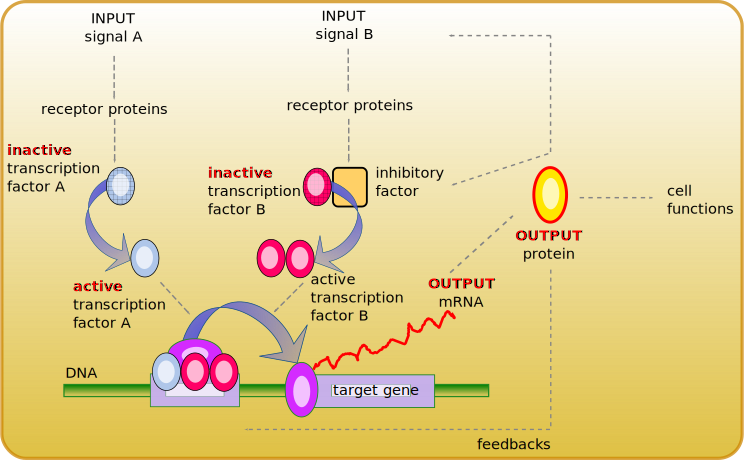
\includegraphics[width=1.3\textwidth]{./Bilder/GRN}
\caption[Transcriptional Gene Regulatory Network (GRN)]{\textbf{Transcriptional Gene Regulatory Network (GRN).}

In this example two different signals have an impact of a single target gene. Signal molecule A triggers the conversion of inactive transcription factor A (green oval) into an active form that binds directly to the target gene's cis-regulatory sequence. The process for signal B is more complex. Signal B triggers the separation of inactive B (red oval) from an inhibitory factor (yellow rectangle). B is then free to form an active complex that binds to the active A transcription factor on the cis-regulatory sequence. The net output is expression of the target gene, leveled by A nd B. Thus cis-regulatory DNA sequences with the proteins that assemble on them, integrate information from multiple signaling inputs to produce mRNA-Output . 
\citep{https://public.ornl.gov/site/gallery/detail.cfm?id=302&topic=&citation=&general=gene20regulatory20network&restsection=all} }
%\setlength{\belowcaptionskip}{0pt} 
\label{fig:Fig.2.}
\end{figure}


\subsection*{Metabolic Interaction}
Metabolic interactions represent the most complex cellular processes. Connections between biochemical reaction via substrate and product metabolites create complex metabolic networks.
The focus is set on the different aspects of enzyme chemistry, enzymestructure and metabolite structure. Thus an individual's metabolism is determined by one's genetics, environment, and nutrition. By investigating the chemical structure of metabolites and systematically classify the functions of the enzymes the understanding of a metabolism and the prediction of enzyme function and novel metabolic pathways is improved.\citep{104(6):1777-1782}\citep{HATZIMANIKATIS2004300}

\newpage

\subsection*{Signal Transduction}

In the developement of multicellular organisms the action of extracellular growth factors activate a cascade of intracellular signaling pathways. These pathways regulate major aspects of cell regulation like cell profileration, cell migration, cell differentiation,cell survival and cell death. To understand the developement of diseases (e.g. cancer) major prozesses (e.g. phosphorylation, ubiquitylation, methylation, etc.) of signal transduction pathways can be delightet by the prediction of a network . In signal transduction proteins are the nodes and directed edges represent interaction, where the biochemical modification of the regulatee is changed by the impact of the regulator. The concentration of signalling pathway underlies high fluctuation over time due to transcriptional and translational regulation, such that the inference of a network is a challenging task \citep{BIES:BIES20834}
%\citep{https://www.ncbi.nlm.nih.gov/pmc/articles/PMC3436851/}.


\begin{figure}[H]
\centering
%\setlength{\abovecaptionskip}{0pt}
\includegraphics[width=0.5\textwidth]{./Bilder/signaltransduction.pdf}
\setlength{\abovecaptionskip}{-10ex}
\caption[Signal Transduction]{\textbf{Signal Transduction.} An environmental signal (e.g. hormone) interacts with a cellular component, most often a cell-surface receptor. The information that the signal has arrived is then converted into other chemical forms, or transduced. The signal is often amplified before introducing a response. Feedback pathways regulate the entire signaling process.\citep{Berg JM, Tymoczko JL, Stryer L. Biochemistry. 5th edition. New York: W H Freeman; 2002. Chapter 15, Signal-Transduction Pathways: An Introduction to Information Metabolism. Available from: https://www.ncbi.nlm.nih.gov/books/NBK21205/} }
%\setlength{\belowcaptionskip}{0pt} 
\label{fig:Fig.1.}
\end{figure}

\subsection*{Protein-Protein-Interaction}
In contrast to the gene regulatory interaction network the protein-protein interactions (PPIs) act directly among themselve. Thus the nodes in a network are the interacting proteins. Proteins interact by physical contacts(e.g. electrostatic forces) of high specificity. PPIs play a big role in electron transfer,signal transduction, transport across membranes and cell metabolism. A variety of techniques are known to detect PPIs. The most applicated ones are immuno-precipitations and the yeast two-hybrid approach. The two-hybrid assay is not a relieable indication that two proteins interact \textit{in vivo},because the two interacting proteins are overexpressed.Thus the interaction may not be present in the wild type cells where the concentrations may be significantly lower. For this reason additional information are included to figure out the occurence of true interaction, such as cellular localization and mRNA expression level. The underlying assumption is that true interactions are likelyto occur between proteinsinvolved in the same biological process, proteins found in the same cell compartment, and proteins whose mRNA are coexpressed.
For the identification of protein complexes affinity purification technique is used followed by mass spectrometry (MS) to sequence the proteins in the complexes. The detection of interactions of protein with DNA is done by chromatin immunoprecipitation (ChIP) in addition with expression microarrays, so-called ChIP on Chip approach. This method provide information about the interaction of transcription factors with DNA and the binding sites of transcription factors. Furthermore computational methods are included to predict the protein interactions by protein fusion and using phylogenetic analysis. Interaction networks of PPIs may depict how drug- protein interactions lead to toxic side effects.
%\citep{10.1371/journal.pcbi.1000807}
\citep{doi:10.1586/14789450.1.2.239}

\newpage
\section{Preprocessing}
%normalization and discretization of the data

\newpage
\section{Boolean Network}
%Define Boolean Network, decribe Definition, give an example
\textbf{Definition: Undirected Graph}\\
In general, an undirected graph $G=(V,E)$ is defined as a set of vertices $V$ describing the nodes of the system and a set of undirected edges $E = \{ (i,j)|i,j\in V\} $ that define a relationship between node $i$ and $j$.\\

This definition can be extended to obtain a notion of a directed graph:\\

\textbf{Definiton: Directed Graph}\\
A directed graph is an ordered pair $G=(V,A)$, defined as a set of vertices $V$ (nodes) and a set of directed edges $A$ (arcs). A set of directed edges $A=\{ (i,j)|\in V\} $ describes the flow of information in the system, where $(i,j)$ describes the flow from $i$ (tail)to $j$ (head). 



\section{Interaction Graph and State Transition Graph}


\textbf{Definition: Interaction Graph}\\
%Definition
%Describe Definition
%Give an example

\textbf{Definition: State transition Graph}\\
%Definition
%Describe Definition
%Give an example
Let $X$ be an \textit{n}-dimensional binary vector that represents the current state of the system. Each element $X_i\in X$ corresponds to the state ($0$ or $1$) of species $i$. A Boolean network defined by a set $F$ of \textit{n} Boolean functions. For every $f_i\in F$, such that $1\leq i\leq n,f_i(X(t))=X_i(t+1)$.\\ 

In other words,given a current state of thesystem $X(t),f_i$ determines the (binary) value of species $X_i$ at time $t+1$. Given a Boolean network $N$ on $n$ variables and an initial state $X(0)\in \lbrace 0,1\rbrace ^n$, the dynamics of the system can be simulated by repeatedly applying the Boolean functions and updating the "current" state.

\textbf{Definition: Boolean Regulatory Network}\\


\citep{10.1371/journal.pone.0066031}%An Evaluation of methods for inferring boolean Networks from time-series data
%---------------------------------------------------------------------------------------------------
A boolean regulatory network consists of nodes (vertices) representing the components of a system and the edges (links) representing  the interaction between the nodes. Each node can take two possible values of 1 (ON) or 0 (OFF). Depending on the input data this could mean, a gene is expressed or not, a transcription factor is active oder inactive, a molecular's concentration is above or below a certain threshold. The edges can be directed or undirected and show the orientation of masstransfer or information respectively. The future state of a node is determined by Boolean rule (function) shown in Figure 1.3. For instance the regulator $v1$ should be inactive such that the regulatee $v2*$ can be active. Here $v2*$ describes the future state of $v2$ \citep{SAADATPOUR20133}. 

\begin{figure}[H]
\centering
%\setlength{\abovecaptionskip}{0pt}
\includegraphics[width=0.4\textwidth]{./Bilder/example02_igraph}
\caption[Interaction Graph]{\textbf{Interaction Graph.} Shown is a selfinvented Interaction Graph constructed in PyBoolNet. The nodes $v1,v2,v3$ are denoted by blue circles, inhibitory arcs are red and activating arc are black. }
%\setlength{\belowcaptionskip}{0pt} 
\label{fig:Fig.3.}
\end{figure}

\begin{equation}
f(v_{1,2,3})= \begin{pmatrix}
 v_1      & \wedge v_2 & \wedge \neg v_2\\
 \neg v_1 &           & \\
         & v_2        &\wedge v_3
\end{pmatrix}
\end{equation} 



Beside the mathematical annotation, the boolean rule can be constructed with the operator AND,OR, NOT or they can be written as \& , ||, ! . The graph in Fig.1. is called the Interaction Graph. Updating the state of a node yield in a network several constellation of states for each node. Regarding the example in Fig.1 for each boolean rule in $f(v)$ all the possible combination of states every node can have is inserted. With $f(v)$ it is possible to determine the next possible state of each node to build an \textit{State Transition Graph}. 
The \textit{State Transition Graph (STG)} is a directed graph representing the dynamical behaviour of a Regulatory Graph. Nodes of this graph represent possible states of the model, assigning a value to each component. Arcs of the STG represent transitions from one state to another. It is an important network to analyze how data behaves over time, thus the most possible state of each component can be computed. But not every state of a component of a node is updated at the same time. Therefore the \textit{State Transition Graph} is either synchronous, updating all the node's states simultaneously, or asynchrounus, the node's states are updated based on their individual timesales\citep{Lee799}. \\\\\newline
Out of the \textit{Interaction Graph} of Fig.1. the synchronous and anysnchronous STG is computed and shown in Fig.2.\\

\begin{equation}
f(v) =  \begin{pmatrix}
 v_1\\
 v_2\\
 v_3
\end{pmatrix}
\textrm{, where }v_{1,2,3}\in\lbrace 0,1\rbrace
\end{equation}

\begin{figure}[h]
  \centering
 \begin{varwidth}{\linewidth}
    \includegraphics[scale=.5]{./Bilder/example01_synchron_stg}
  \end{varwidth} % ein Leerzeichen Abstand
  \begin{varwidth}{\linewidth}
    \includegraphics[scale=.4]{./Bilder/example01_asynchron_stg}
  \end{varwidth}
  \caption[Synchronous and Asynchronous State Transition Graph]{\textbf{Synchronous and Asynchronous State Transition Graph}. Left: Synchronous State Transition Graph; Right: Asynchronous State Transition Graph}
\label{fig:Fig.4.}
\end{figure}

%----Mathematische Definition von synchronen und asynchronen Update
\citep{REMY2008335}

\section{Network Evaluation}
%Define Accurancy, Precision, Recall, ROC, AUC


    %\clearpage{\pagestyle{empty}\cleardoublepage}		% l�scht Kopfzeilen und Seitennummerierung von der letzten Seite eines Kapitels, sofern dort kein Text mehr steht
    \chapter{Materials and Methods}
\section{Inferencealgorithms}
%Baysian networks,Boolean regulatory networks, Ordinary differential equation models and Neural networks
regression
\citep{CHAI201455}
%Welche Algorithmen gibt es?
%Warum wählen wir hier den Boolean Approach?
\subsection*{Boolean Approach}
%Define REVEAL, BESTFIT und FULLFIT 
\subsection*{Baysian networks}
\subsection*{Ordinary differential equation models}
\subsection*{Neural networks regression}
BIBN (Bayesian inference approach for a Boolean network)
REVEAL (Reverse Engineering algorithm)
PCA-CMI (Path consistency algorithm- Conditonal mutual information)
ARCANE (Time-delay algorithm for reconstruction of accurate cellular networks)
MIDER (Mutual information distance and entropy reduction)\citep{MIDER}
	defines a mutual information based distance between genes to specify the directionality
BESTFIT ()

These mutual information-based methods are computationally expensive, because they are implemented to compute exact mutual information values over all possible combinations of genes.

RelNet (Revelance network algorithm)

CLR (context likelihood of relatedness method)
CST (chi-square test)

\section{PyBoolNet}



\section{Data Selection}
\subsection{Example data set}
%How the example data set is created
%
\subsection{HPN-DREAM breast cancer data set}
Now it is shown how the Pipeline can be applied to a real-life time course data set. 
\subsubsection*{What is the Dream Challenge?}
For a Boolean network inference the data of a platform so-called Dialogue on Reverse Engineering Assessment and Methods (DREAM) - Challenge is used. The DREAM-Challenge is a non-profit, collaborative community effort consisting of contributors from across the research spectrum of questions in biology and medicine. This organization was built in 2006 and publishes crowdsourcing challenges with transparent sharing of data, thus everyone can participate the challenge. The DREAM-Challenge has partnered with Sage Bionetworks, which provide the infrastructure by Sage Bionetworks Synapse platform to get access to the open collaborative data analysis. Overall the DREAM-Challenge is a helpful instrument to get real-life data, comparing results and interact with other researchers all over the world, while contribute solutions to biological and medical questions.\citep{DreamChalleneg Homepage}.
The challenging question was to decide which Dream Challenge data set could be useful for this masterthesis. For inferring a Boolean network and further analysis of the state tarnsition graph the desired data set should contain measurements of experiments with less pertubational information and a in a time course context. 
The Dream Challenge 5 dealing with gene-gene interaction,providing test and training data sets of gene expressions seemed to be an appropriate candidate. But there was less time course information and a high abundance of pertubation. Thus the Dream8 Challenge is was chosen. This challenge describes protein-protein interaction and measurements for multiple timepoints.

\subsubsection{DREAM8}
%Short sentence about the DREAM8 Challenge: What is the goal(medically and mathematically)?What sub challenge do I do?

\subsubsection*{Data Collection}
The collection of the HPN8 breast cancer PPI data is done by a technique so called Reverse phase protein array(RPPA). This technique is divided up into 6 parts:
\subparagraph*{Sample collection}
%Wo kommen die breast cancer cells her?Erwähne: Es gibt 4 Zelllinien (BT20, UACC812, BT549, MCF7) und 8 Stimuli (Insulin, Serum, HGF, NRG1,EGF, FGF1,GF1,IGF1), welche am Ende 32 Netzwerke ergebe. Vielleicht die Zelllinien und die Stimulis erklären.
An inhibitor or stimulus in form of drugs is added to a set of celllines at the same time and the celllines are then processed at different time points.
\subparagraph*{Cell Lysis}
Cell fragments are lysed with a celllysis buffer to obtain high protein concentration.The choice of a buffer decides the quantity of proteins can be lysed out of the cell.
%Welche buffer wurden in der Dream Challenge verwendet.
\subparagraph*{Dilution}
Dilution of the celllysed probes.
\subparagraph*{Antibody screening}
The lysates are pooled and resolved by SDS-PAGE followed by western blotting on a nitrocellulose membrane. The membrane is cut into 4mmm strips. Each slide is probed with a  different antibody, primary with a secondary antibody.
\subparagraph*{Fluorometric detection}
Primary and secondary antibody are diluted.%with which buffer?TBST?%
Detection reagentisput on each slide. Signal amplification and detection is done by an optical flatbed scanner if colormetric technique is used orby laser scanning. %Welche methode wurde verwendet?
\subparagraph*{Data set structure}
Missing data points and outliers are detected and deleted from the data set. The data set is normalized %Welche Struktur weißt der Datensatz am Ende auf? Welche Informationen sind davon für uns wichtig? Normalisierungalgorithmus wurde hier verwendet?




    \clearpage{\pagestyle{empty}\cleardoublepage}
    \chapter{Pipeline and Results}
This chapter introduces the pipeline of the \textit{in silico} data set (Figure 3.3, Figure 3.8) and the pipeline for the Dream8 Challenge data set describing the processing of the data from discretization to inferring a network and finally scoring the predicted network against a gold standard network. The results of the \textit{in silico} data set are necessary to set the paramter for the Dream8 Challenge pipeline. Both pipelines can be executed from the command line by a bash script and are available on Git: "github.com/ninakersten/Masterthesis". 

\section{Pipeline of the \textit{in silico} data set}

For both the subnetworks and the cell cycle network continous data sets ($S=\{ S_{1},S_{2},...,S_{n}\} $) are generated with \textit{odefy}, a MATLAB- and Octave-compatible toolbox for the automated tansformation of Boolean models into systems of ordinary differential equations \citep{Krumsiek2010}. With \textit{odefy} the number of sample points and the time interval for a data simulation can be determined. The time interval is set to a range of 1 to 50. For later application of the Dream8 Challenge data set the \textit{in silico} data sets are converted into the CSV format in the structure of the Dream8 Challenge input data (Table 2.8) and for the discretization and learning step converted into a text file format (Figure 3.1). The species' names are anonymized by single character depicted in the first header of a \textit{txt} file and original names are stored in a header below followed by the time course data set \textit{S}.

%\noindent See the following command :
%\begin{lstlisting}[language=bash]
%  $ bash insilico.sh 100 KM3 BESTFIT
%\end{lstlisting}

%bild zeigen, wie die Daten in dem file angeordnet sind.
\begin{figure}[H]
\captionsetup{width=1.0\linewidth}
\centering
\includegraphics[width=1.0\textwidth]{./Bilder/CSV2TXT.pdf}
\caption[CSV to TXT]{\textbf{CSV to TXT:} Anonymized single character represent the species and information about cell line,inhibitor and stimulus is neglected. }
\label{fig:9}
\end{figure}


After discretizing continous time course data into a set of binary values ($B=bin(S)$, where $bin\in \{ $2-k-means, iterative k-means$\}$) redundant values are removed from this set. Boolean networks ($N=learn(B)$) are learned from this data by each inference algorithm ($learn\in \{$Best-Fit, Full-Fit, Reveal$\}$). A value for the minimal error $MinError$ is set, sucht that the inference algorithms runs i times until a network with an error ($Error(N,B)$) lower that the minimal error is achieved. It is worthwhile to get an error of $0$, meaning the the boolean model describes the data perfectly. The amount of returned solutions is set to a value of $3$, such that in each inference process three solutions (resp. Boolean Networks) are inferred, all with an error lower than the minimal error. A single Boolean Network with the lowest error across all iterations is selected for further processing.\\
For investigating the impact of the \textit{in-degree} in a network on the algorithms performance, the E.Coli subnetworks are processed by the iterative k-means clustering algorithm with a cluster depth of $d=3$ in combination with Best-fit, Full-fit or Reveal. The cluster depth with $d=3$ is selected due to previous research proving its reliablity regarding the trade off between simplicity and loss of information (e.g. oscillations).\\
%Quelle: TS2B Paper
For assessing the dependence of an inference algorithm to the number of sample points, the continous data for the cell cycle is generated for $m\in\{ 50$, $100$, $150$, $200$, $250$, $300$, $350$, $400$ ,$450$, $500\}$. Starting by a number of 50 sample points is due to the fact, that with lower amount the inference algorithms can not run. And for measuring the impact of the clustering depth the cell cycle's continous data is generated with 100 sample points (similar to the abundance of sample points of $\sim 85$ in the Dream8 Challenge) and inferred with a clustering depth of $d=\{ 1,2,3,4,5,6,7,8,9,10\}$. In Table 3.1 shows a summerized overview of these settings.

\begin{table}[H]
%\resizebox{\textwidth}{!}{
%{\tabcolsep=6pt%
\begin{center}
%\captionsetup{width=0.87\linewidth}
%\small
\begin{tabular}{l|l|l}
\toprule 
 & E.coli & Cell cycle \\
 \hline\hline
\# networks & $45$ & $1$\\
\rowcolor{black!10} \# nodes & $\{10,11,12,13,14\}$ & $10$\\
max. \textit{indegree} & $\{1,2,3,4,5,6,7,8,9\}$ & $5$\\
\rowcolor{black!10} \# sample points & $100$ & $\{50,100,150,200,250,300,350,400,450,500\}$\\
cluster depth & $3$ & $\{1,2,3,4,5,6,7,8,9,10\}$\\
\rowcolor{black!10} Best-fit & \checkmark & \checkmark \\
 					Full-Fit & \checkmark & \checkmark \\
\rowcolor{black!10} Reveal & \checkmark & \checkmark \\
\bottomrule
\end{tabular}
\captionof{table}{\textit{In silico:} Setting Table}
\end{center}
%}
\end{table}  

The predicted networks are converted (from bnet format) to interaction graphs (to a sif format) by PyBoolNet (Figure 4.2). Each predicted interaction graph is scored against a gold standard interaction graph generated from the initial boolean network with PyBoolNet. Hence each line in a SIF-format of an interaction graph represents an edge of the graph (Figure 4.2). The edges of the gold standard and the prediction are compared resulting in a confusion matrix for computing Precision, Recall, Accuracy, Balanced Accuracy and the Matthew Correlation Coeffiecient.

\begin{figure}[H]
\centering
\includegraphics[width=0.7\textwidth]{./Bilder/bnet2sif.pdf}
\caption[Boolean Network to Interaction Graph]{\textbf{Boolean Network to Interaction Graph:} The predicted Boolean Network $N$ is converted into the Interaction Graph $IG$.}
\label{fig:9}
\end{figure}

 

\begin{figure}[H]
\centering
\includegraphics[width=0.55\textwidth]{./Bilder/pipeline_insilico.pdf}
\caption[\textit{In silico} Pipeline]{\textbf{Pipeline \textit{in silico}.}}
\label{fig:9}
\end{figure}



\section{Results of the \textit{in silico} data set}
\subsection*{In-degree}
The subnetworks of E.Coli are grouped into nine categories, each containing five subnetworks with 10,11, 12, 13 and 14 nodes. A category denote the number of incoming links (resp. in-degree) of each node in a network. The Figure 4.4 shows the scoring result of the 45 subnetworks by the average structure accuracy. Increasing the in-degree causes an decreasing of the accuracy. 

\begin{figure}[H]
\centering
\includegraphics[width=0.9\textwidth]{./Bilder/Scoring/insilico/1_Indegree_Runtime/MeanAcc_indegree.pdf}
\caption[Average Structure Accuracy]{\textbf{Average Structure Accuracy.} E.Coli subnetworks are grouped into nine groups definded by the in-degree of the nodes in a subnetwork. With increasing in-degree the average accuracy of all three inference algorithms decreases. }
\label{fig:}
\end{figure}



Thus the more nodes occure with a high in-degree the more complex is the system and the worse the inference algorithm is able to detect the whole information. This observation covers the observation of \citep{10.1371/journal.pone.0171097}, where the settings where slightly different. instead of grouping sets of networks, they grouped the nodes of about 300 networks with different network sizes ($|V| = 10,20,$...$100$).\\

\subsection*{Number of sample points}
For the cell cycle continous data different sets with different number of sample points $\{50,100,150,200,250,300,350,400,450,500\}$ are generated. The resulting networks are tested by accuracy, precision, recall and Mathew correlation coefficient. The Figure 4.5 shows that changing the amount of sample point does not change significantly the performance of the algorithms.

\begin{figure}[H]
\centering\includegraphics[width=0.9\textwidth]{./Bilder/Scoring/insilico/2_cellcycle_measurements/RecPrec.pdf}
\caption[NumberOfPoints]{\textbf{Number of sample points.}In (a) the accuracy ranges around a value of $0.7$, whereas Precision (c) and Recall (d) range on a low level of $0,3$ to $0,4$. Despite a few insignificant fluctuations the value almost alway stays the same. In (b) the mcc does not change either.}
\label{fig:}
\end{figure}

\begin{figure}[H]
\centering\includegraphics[width=0.9\textwidth]{./Bilder/Scoring/insilico/2_cellcycle_measurements/Bacc.pdf}
\caption[NumberOfPoints]{\textbf{Number of sample points.}In (a) the accuracy ranges around a value of $0.7$, whereas Precision (c) and Recall (d) range on a low level of $0,3$ to $0,4$. Despite a few insignificant fluctuations the value almost alway stays the same. In (b) the mcc does not change either.}
\label{fig:}
\end{figure}

\subsection*{Cluster depth}
Changing the cluster depth of the iterative k-means clustering algorithm changes the performance of the algorithms not significantly. As mentioned in (Paper),the iterative k-means clustering algorithms captures the oszillations (resp. kind of dynamic) in a system in contrast to the two cluster k-means algorithm. Beside the fact only the structure of a network not the dynamics are analyzed later network inference is performed with the iterative k-mean clustering method with a recommanded clustering depth of $d=3$ (Paper).
%Paper of TS2B
\begin{figure}[H]
\centering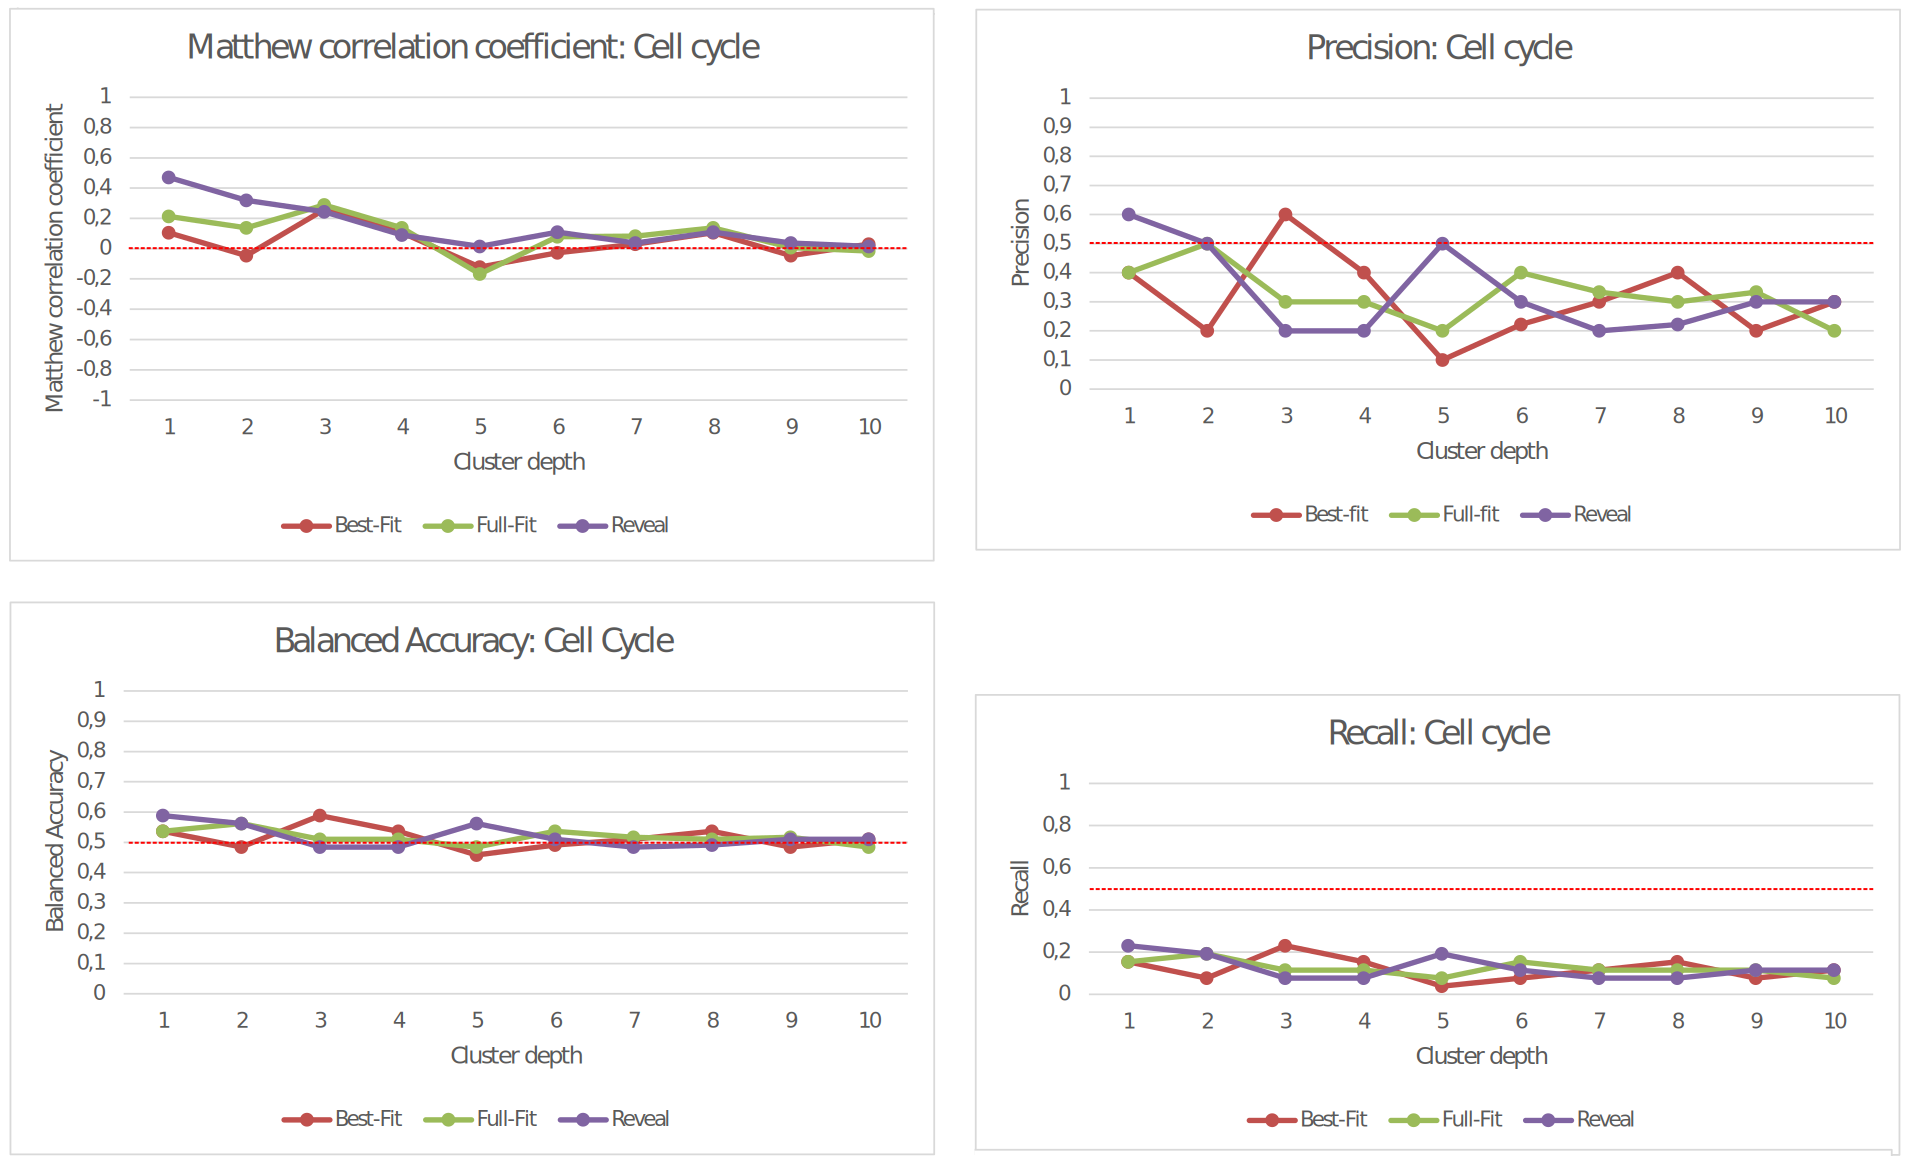
\includegraphics[width=1.0\textwidth]{./Bilder/Scoring/insilico/3_cellcycle_clusterdepth/insilico3.pdf}
\caption[Clusterdepth BCC]{For a clustering depth of $1$ to $10$ the three algorithms are performed resulting in a balanced accuracy that ranges around a value of $0,5$. Changing the clustering depth causes no significant change in the network performance.}
\label{fig:7}
\end{figure}

\section{Pipeline of the Dream8 Challenge data set}
\begin{figure}[H]
\centering\includegraphics[width=0.6\textwidth]{./Bilder/pipeline_dream8.pdf}
\caption[pipelineDream8]{\textbf{Pipeline Dream8 Challenge. }}
\label{fig:9}
\end{figure}

%Raw structure
%-Pipeline fast identisch in silico pipeline mit einzigen Unterschied: input datensatz, km3+bestfit und gold standard selection.

%Learn-method: BESTFIT wird benutzt, weil: aus in silico weiß man, dass es mit fullfit gleich auf ist und durch das TS2B Paper, dass es die beste performance hat. 
% Prediction is converted to .bnet format for .sif format
%Goldstandard: welchen goldstandard hat die challenge verwendet und welchen gold standard benutze ich?
% Scoring gegen Prior aggregated network, aggregated network und letzten aus dem leaderboard(soll zeigen, dass Daten unbalanced sind), Erklären, warum ich mein eigenes Scoring mache und nicht dreamtools verwenden kann.
%Threshold: Wenn ich mehrere solutions habe, dann edge score berechenen über die Häufigeit von auftretenden Kanten, dann threshold verschieben, sodass von wenig bis viele tp sich ergeben = AUROC / = AUPR (Wegen runtime nicht gemacht,aber ich dann es ja für nur 3 runs zeigen?)


%Create 32 data set from training data -> txt. file
The 'main' training data set of the Dream8 Challenge is converted into a text file format (Figure 2.8, Figure 3.1) by splitting each data set of a cell line into eight text files depending on the stimulus. Each of the resulting 32 text files contain about $\sim $85 sample points and about $\sim $45 antibody names (Figure 3.8).\\

\subsection*{Network inference}
%Quelle: TS2B Paper mit KM3 Empfehlung
%The python implementation of the inference algorithms is validated, such that a network up to 50 nodes can be inferred and the 
%Network inference: KM3+Best-Fit
The higher the \textit{in-degree} of the nodes and the amount of nodes in a network the higher is the complexity in a system and the higher is the computational cost of an inference algorithm. Due to computational limitations and a technical settings of 8 RAM and a Core i5 processor the application of Reveal to the Dream8 Challenge data set is an infeasible task. 
Furthermore, results of the \textit{in silico} data set show that the choice of cluster depth abundance of sample points have no significant influence on the performance. An increasing \textit{in-degree} shows an decreasing performance for all three algorithms, such that no algorithm can be excluded by this investigation. Thus, results of (Paper Quelle) regarding error assessment are taken into account, such that a recommanded combination of Best-Fit with the iterative k-means algorithm with a $d=3$ is applied to the Dream8 Challenge data set. This combination yielded the best performance , especially in complex systems.\\
Predicted Boolean networks (\textit{bnet}) are converted into an Interaction graph (\textit{sif}) (Figure 4.2) and scored against a gold standard (Aggregated Network, Prior Aggregated Network). 
%Paper:TS2B Paper 
%Mit Fullfit auch das Scoring machen.

\subsection*{Gold standard selection}
%Goldstandard der challenge 
%Wie wird in der challenge gescored und (testdatensatz und AUROC AUPR, und wie score ich: Aggregated Network, Prior Aggregated Network, kein kantengewicht, kein threshold, daher Recall, Precision,....)
Network inference methods are often assessed using data simulated from known causal network structure, so called "gold standard network". It is useful to include prior knowledge, but this can come along with limitations, because it is difficult to truly mimic specific bilogical systems of interest. Learning novel connections in a network is restricted by comparing inferred networks to literature. For this purpose no gold-standard is provided in this Dream Challenge.  For testing the algorithms an \textit{in silico} data set is provided and prior knowledge independent network can be created with the training data set of the experimental data. The \textit{in silico} data set is generated from a nonlinear ordinary differential equations (ODE) model of the ERBB signaling pathway (ERBB:family of proteins containing four receptor tyrosine kinases, structually related to the epidermal grwoth factor receptor (EGFR)). Nevertheless pre-existing biological knowledge was included by several participants and seemed to be broadly benefical. The predicted networks from the training data were assessed by the test data.
After finishing the challenge an Aggregated Network for all 32 contexts was submitted. These aggregated networks are a compendium of 66 submissions of the participants of this challenge with the best performance reduced by correlated submissions.
%Paper: Dream8 Challenge über aggregated networks
Furthermore an Aggregated Prior Network is provided, a combination of 10 prior knowledge networks that teams used as part of their submission (Table 3.2). Hence, the aggregated network and the aggregated prior knowledge network are used in this thesis as a gold standard to test the performance of Best-Fit. Predictions of all 74 participants of the Dream8 challenge leaderboard are scored against the two aggregated networks,such that a new ranking including the new prediction by Best-Fit is determined.

\begin{table}[H]
%\resizebox{\textwidth}{!}{
%{\tabcolsep=6pt%
\begin{center}
%\captionsetup{width=0.87\linewidth}
%\small
\begin{tabular}{l|l|l}
\toprule 
Network & $\# $ Edges & $\# $ Networks\\
 \hline\hline
Prediction (Best-Fit) & $\sim 140$ & 1\\
\rowcolor{black!10} Aggregated Network & $\sim 2200 $ & 66\\
Aggregated Prior Network & $\sim 1400$ & 10\\
\bottomrule
\end{tabular}
\captionof{table}{Network structure}
\end{center}
%}
\end{table} 



\subsection*{Evaluation}
Due to different strategies of evaluating predictions, e.g. choice of the scoring metric and implementation approach, it is hard to compare the resulting performance between the participants. For this reason the Dream8 Challenge provides a standard scoring tool 'DREAMTools' Python package.
%Quelle:  \citep{Cokelaer T, Bansal M, Bare C et al. DREAMTools: a Python package for scoring collaborative challenges [version 2; referees: 1 approved, 2 approved with reservations]. F1000Research 2016, 4:1030 (doi: 10.12688/f1000research.7118.2)}
This tool needs as input a \textit{sif} and an \textit{eda} file, where eda (electronic design automation) contains the confidence scores of edges in an Interaction Graph. By these information dreamtools returns AUROC (area under the receiver operating characteristic curve)  and AUPR (area under the precision recall curve). AUPR is used for the case when there is an imbalance in the classes of the confusion matrix. Here a threshold $\tau$ is shifted, such that the true positiv value increases and a curve for both metrics are producible.
%Verweis auf Anhang: Erklärung/Definition von AUPR und AUROC
An idea is to run the pipeline several times, ideally about 100 times to get a sufficient set of confiodence score for the prediction. Then over the resulting set of predictions occurences of edges are count, such that a pobability of an edge occurence is obtained. As mentioned in 'Network inference' the computational power is limited. One execution of the pipeline needs about 5 hours. Of course it was taken into account to use a cluster (e.g. Allegro), due to a lack of globally implemented bioconda for installing Pycluster, this approach failed.
Therefore, just the performance of the algorithms concering inferring the interaction graph is performed, such that the scoring tool of the DreamChallenge can not be used. For this reason an own scoring script is implemented by comparing the interaction graph of the prediction against a gold standard returning the precision, recall, structural accuracy, balanced accuracy and Matthew corrlation coefficient. 

\newpage
\section{Results of the Dream8 Challenge data}
\subsection*{Prediction versus Aggregated Network and Aggregated Prior Network}
Scoring the prediction against the last participant of the leaderboard in the Dream8 Challenge (rank: 74.) ranges in the accuracy inbetween a value of 60\% to 80 \% (Figure 4.8). Scoring the prediction against the aggregated network yields are accuracy of 10\% to 18\%. This is du to the fact, that the cases of true negatives and true positives have a high imbalance. The application of the balanced accuracy shows that the previous observation has no significance of the performance.  
% High amount of FalseNegatives: Bad accuracy for prediction against aggregated network
% High amount of TrueNegatives: Good accuracy for prediction against aggregated network
%= Yield: Balanced accuracy is at random.
%Vllt. noch prediction vs. prior knowledge network mit einfügen
\begin{figure}[H]
\centering
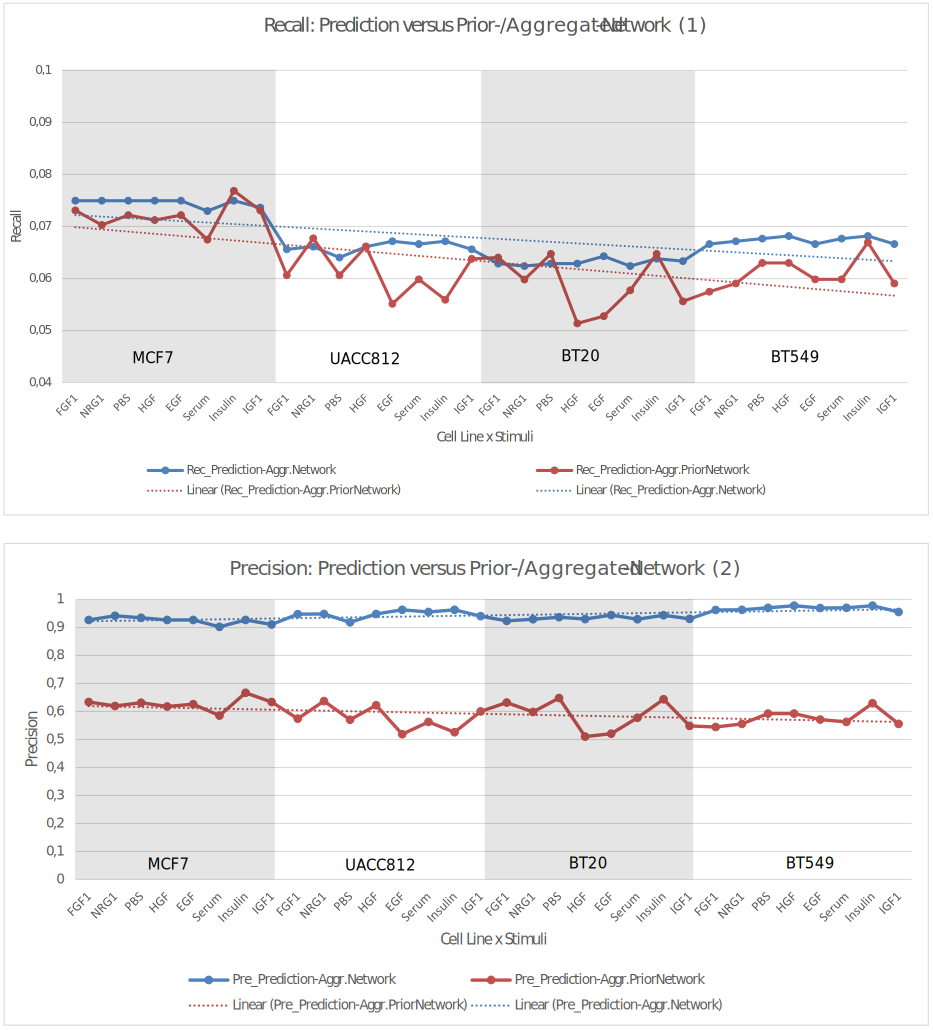
\includegraphics[width=1.0\textwidth]{./Bilder/Scoring/dreamchallenge/1_Balanced_vs_Unbalanced/balanced.pdf}
\caption[Blanced vs. Unbalanced]{Balanced versus Unbalanced. Accuracy and Balanced Accuracy for (1) Prediction scored against Aggregated Network and Aggregated Prior Network; (2) Prediction scored against Aggregated Network  and submission of the 74. participant of the Dream8 Challenge.}
\label{fig:10}
\end{figure}

\begin{figure}[H]
\centering
\includegraphics[width=1.0\textwidth]{./Bilder/Scoring/dreamchallenge/1_Balanced_vs_Unbalanced/balanced_rec_prec.pdf}
\caption[Recall and Precision: Prediction versus Aggregated/Prior Network]{Recall and Precision: (1) Prediction versus Aggregated Network and (2) Prediction versus Aggregated Prior Network}
\label{fig:10}
\end{figure}

\subsection*{New Ranking: Aggregated Network and Aggregated Prior Network}
%New ranking
%Noch scoring für: MCC für prediction + submissions gegen aggregated prior knowledge network

\begin{figure}[H]
\centering
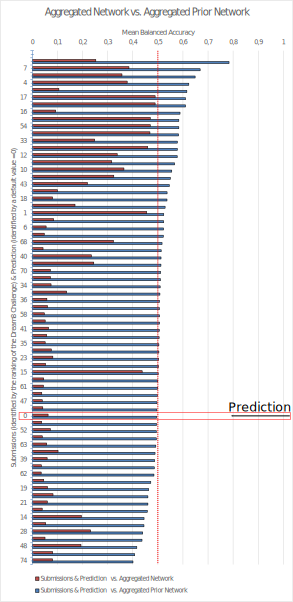
\includegraphics[width=0.62\textwidth]{./Bilder/Scoring/dreamchallenge/Meanbacc_vertical_comparison.pdf}
\caption[New Ranking (Balanced Accuracy): Aggr. Network and Aggr.Prior Network]{New Ranking: Aggregated Network and Aggregated Prior Network}
\label{fig:}
\end{figure}


%Hier noch precision,recall, acc, bacc einfügen?
%Angeben welchen Platz diePrediction nach dem neuen Ranking hätte
%scoring der prediction gegen das AggregatedPrior Knowlede network





    \clearpage{\pagestyle{empty}\cleardoublepage}
    %\chapter{Results}



\section{}

\begin{figure}[H]
\centering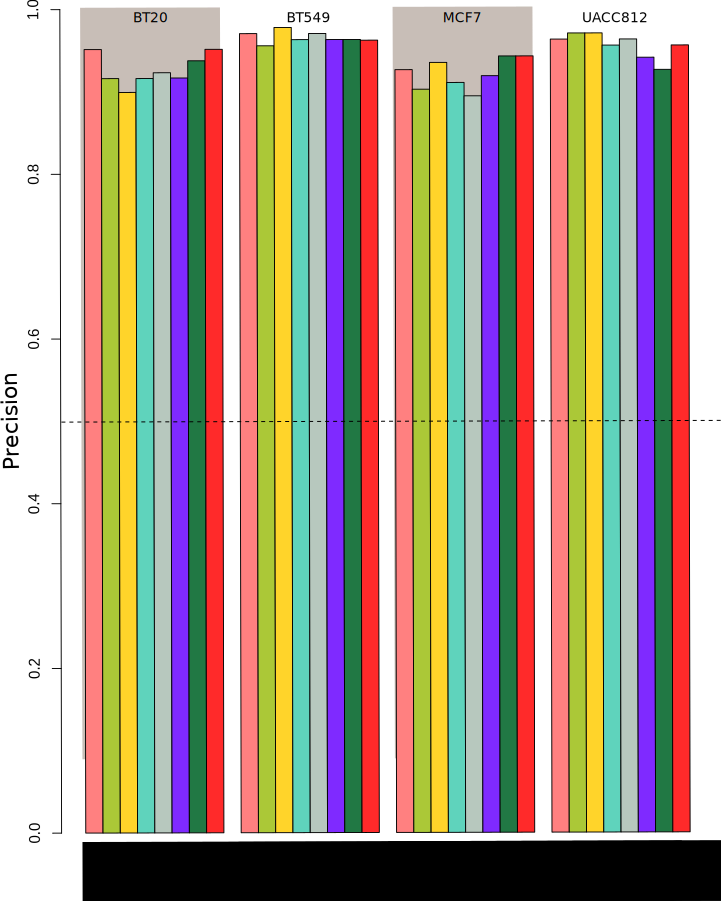
\includegraphics[width=0.4\textwidth]{./Bilder/Precision.pdf}
\caption[Precision]{ }
\label{fig:}
\end{figure}


\section{}


\section{}


    %\clearpage{\pagestyle{empty}\cleardoublepage}
    \chapter{Discussion}
%Preprocessing

%TS2B:%Quelle: TS2B-Paper/ Error-Assessment-Paper

%Nachteile von BooleanModels:
%- Recent survey say: "Faithfulness to biological reality", "ability to model dynamics"is low
%- TS2B needs a relatively large number of time points in the time-series data, otherwise we have the problem of "too many variables, too few equations", which a very large degree of freedom, thus a nonuniqueness of solutions.
%- In practice the regulatory network is unknown, thus judging whether a BN provides a close approximation or notis not easy.
%- ODE's are used to simulate the "true dynamics", but ODE's are not necessarily unique with respect to the dynamics they generate
%- It is important to mention,that often the goldstandard network is constructed from multiple informtion (literature, mature information).In this case just the raw time-series data was provided without additional information.
%- Parameter of the model have a big effect:e.g. Initial concentration in the time-series data set: Has significant influence on the topology and functions of the inferred BN. For instance: if the reaction rate is quite low the dependecy of two genes cant be observed in the synchronous documented time-series.
%-\citep{CHAI201455}: BN-based methods are not suitable for large-scale network inference,because allpossible combinations of genes were exhaustivley compared so as to find a best of regulatory genes for a given target gene. (e.g. Bestfit, REVEAL)

%Vorteil:
%- Very closely reflecting the topology of a regulatory network (upstream/downstream relationships)
%- faithfulness to biological reality: Binarization, redundancy removal -> varying degrees
%- number of Boolean functions is exponential in the number of genes in the system

%General:
%- The more complex a system is (heavily oscillatory,large variability) the more time points are needed.
%- BN have a good predictive power for small networks
% Fast convergence of BESTFIT can be explained by its lack of requirement that the candidate functions f' be complete.
% Slow Convergence: REVEAL only accepts complete functions, thus R. produces more intuitive BN


%Finally:
%- The amount of time-points at which concentrations maust be sampled may be very large (with disagrees with commonly stated claim that BN require very little data to learn or train.)

%Improvements & Outlook:\citep{CHAI201455} 
% - There are several other boolean algorithms for network modeling:
% - Baysian inference approach for a Boolean Network(BIBN): The maximum number of regulatory genes is bounded by two and used to infer a Boolean network by maximizing a joint posterior probability. To select the most informative regulatory genes an approximated multivariate mutual information measure is inccorporated.
%- ARCANE: Time-delay algorithm for the reconstruction of accurate cellular networks (ARCANE) method is used to compute the mutual information by considering a time gap between gene expression values.\citep{Zoppoli2010}
%MIDER: Mutual information distance and entropy reduction method (MIDER),which defines a mutual information-based distance between genes to specify the directionality.\citep{10.1371/journal.pone.0096732}
%- MIBNI: Mutual information-based Boolean network inference method:The method first identifies a et of initial regulatory genes using mutual information-based feature selection, andthen improves the dynamics prediction accurary by iteratively swapping a pair of genes betweensets of the selected regulatory genes and the other genes. (good for structural and dynamic analysis)\citep{10.1371/journal.pone.0171097}
%- Kombination aus Boolean Approach und ODE: First break down the complex system to low level informative network. Attractor analysis. Then focus on the nodes of the attractor and the basinsand then just look by ODE on the smaller subset of nodes.(e.g. kinetic information)

%- GROßER NACHTEIL:
%These mutual information-based methods are computationally expensive, because they are implemented to compute exact mutual information values over all possible combination of genes.

%Quelle: https://www.nature.com/articles/nmeth.3773
%- In insilico data network inference were almost better inferred when teams did not use prior knowledge.
%- Conversely, notusing a prior network did not necessarily result in poor performance; mean AUROC scores ranged from 0.49-0.71, with prior knowledge: 0.49-0.78.
%- Similar previous DREAM challenges showed that there is no clear relationship between method (inference algorithm) and performance. Pre-processing and implementation are important.
%- With the aggregated prior network potentially novel changes can be highlighted.
%- Although causal network inference mayfail for many theoretical and practical reasons, the results of this challenge showed, that it is feasible inferring significant large-scale networks in complex mamalian settings by a community effort.
%- it is emphasized that further work needed to clarify the theoretical properties of the score.
%Result: Their analysis revealed contexts that deviate from known biology, such deviations are likely to be particularly important for understanding disease-specific dysregulation and therapeutic heterogenity. Furthermore, it is possible that the literature is biased toward cancer, and for that reason priors based onthe literature may be less effective in other disease settings.

% DREAM Challenge:Additional Data Details
% Quelle:https://www.synapse.org/#!Wiki:syn1720047/ENTITY/56210
% - Some phopsho antobodies have low quality and should be xcluded from the set
% - Annotation error might cause wrong scoring against the gold standard
% - Antibodies are NOT comparable. Each antibody has varying degrees of affinity and avidity towards its target protein. Assuming two proteins have the same concentration, they may not result in the same level of data values. Therefore, they are not directly comparable.
% - Batch Effect: Samples in different cell lines are NOT comparable (e.g. the datapoint for AKT_pS473 in MCF7 (serum,5min,DMSO) can not be compared with the corresponding datapoint in BT20).Normalization procedures could be used to reduce the batch effect.
% - The antibodies available for this assay have evolved over time, so the proteins measured are not identical across all datasets. (BT20 = 48, BT549 = 45, MCF7 = 41, UACC812 = 45 phophoproteins)
% - Some antibodies target more than one isoform of a protein (eg: the antibody for AKT targets AKT1, AKT2, AKT3)


%-Normalization of microarray data important: Choice of normalization method important
    \clearpage{\pagestyle{empty}\cleardoublepage}

% -----------------------------------
%\backmatter 
%\bibliographystyle{abbrv}
\renewcommand{\bibname}{References}
\bibliographystyle{unsrt}				% bei natbib in deutsch
{\footnotesize\bibliography{./Literatur/quellen4}}		% Literaturquellen einbinden  			
\appendix

\chapter{Appendices}
\section{DREAM8-Challenge scoring priciples}

For determining the Receiver-Operating-Characteristic-Curve a True-Positive-Rate (TPR) and a False-Positive-Rate (FPR) is calculated.\\
\begin{defn}\textbf{True-Positive-Rate (TPR).}\\
\textit{The TPR values are for the y-axis of the ROC.}
\begin{equation}
TPR=\frac{TP}{TP+FN}
\end{equation}
\end{defn}
\begin{defn}
\textbf{False-Positive-Rate (FPR).}\\
\textit{The FPR values are for the x-axis of the ROC.}
\begin{equation}
FPR=\frac{FP}{FP+TN}
\end{equation}
\end{defn}

Threfore, a threshold $\tau$ is set and the confidence scores are classified by this threshold.  Confidence scores below this threshold take a value of $0$ indicating an edge is less likely to occur and a confidence score above $\tau$ is taking a value of $1$ indicating an edge is potential. By increasing the threshold $\tau\in[0,1]$ the amount false positve decrases and false negative increase. 
Resulting calasses are put into a context of True Positive Rate ($TPR=\frac{TP}{TP+FN}$) and False Negative Rate ($FPR=\frac{FP}{FP+TN}$). This yields a set of values returning a value of the area under the receiver operating characteristic curve (AUROC).\\\\   
Similar to balanced accuracy the AUPR (area under the precision recall curve) metric is used for imbalanced classes in the confusion matrix taking precision and recall in relationship by shifting $\tau$.



\end{document}
